\documentclass{SSBT-BE}
\usepackage{makeidx}
\usepackage{amssymb}
\usepackage{float}
\usepackage{amsmath}
\usepackage{subfigure}
\usepackage{ragged2e}
\usepackage{%
  babel,
  algorithmic,
  algorithm,
  caption
}

\usepackage{url}
\usepackage[breaklinks=true]{hyperref}

\usepackage[intoc]{nomencl}
\renewcommand{\nomname}{Abbreviations}
\makenomenclature
\makeindex
\begin{document}
\title {VIRTUAL LAB ASSISTANT }
\author{\\ Pradnya Vijay Nikam 
        \\ Chhayashree Pralhad Patil
       \\ Gauri Vijay Sonar
       \\Saniya Javed Shaikh
       }
\dept{Department of Computer Engineering 2024-25}
\supervisor{Dr.Akash.D.Waghmare }

\degree{Bachelor of Engineering}
\specialization{Computer Engineering}
\type{Minor Project}
%\type{Seminar}
\hod{Dr. Manoj E. Patil}
\submitdate {2025-26}
\beforepreface 

\afterpreface
\listoffigures
\newpage
\listoftables
\newpage
%\input{glossary}
\clearpage
\pagenumbering{arabic}
\pagestyle{plain}

\prefacesection{Acknowledgements}
%\input{acknowledgement}
No work could have been accomplished without the cooperation, guidance, and support of many individuals. The team members express their heartfelt gratitude to everyone who contributed to the successful completion of this project. Many thanks are extended to the almighty God for providing the strength and determination to undertake this endeavor.
We are deeply grateful to Principal Prof. Dr. Girish K. Patnaik for providing the necessary resources and a supportive environment for our academic pursuits. Our sincere gratitude also goes to Dr. Akash D. Waghmare, Associate Professor, for his insightful suggestions and continuous encouragement, which were instrumental in completing this project.
Special appreciation is reserved for Mr. Ashish T. Bhole, Associate Professor, who served as the TE Project Incharge. His role exemplified exceptional dedication, as he provided expert guidance, constructive feedback, and continuous motivation throughout the project duration. His support and mentorship were pivotal in helping us achieve our objectives and enhance the overall quality of our work.
Acknowledgments are also extended to the faculty members and lab assistants who provided technical support, as well as our peers for their collaboration and encouragement. Lastly, we express our deepest gratitude to our parents and friends for their unwavering support and understanding, which enabled us to persevere and successfully complete this project.





\acknowledgeauthor

% Use following command at the command prompt to display the Abbreviations
 %makeindex thesis.nlo -s nomencl.ist -o thesis.nls
  \makeindex
 
\prefacesection{Abstract}

The Virtual Lab Assistant is a web-based system designed to conduct and manage practical examinations in a digital environment. 
The system provides features such as student authentication, practical selection, real-time query evaluation, and performance tracking. 
Each student logs in using a unique credential, ensuring secure and controlled access to the system. 

The platform allows students to perform practical tasks by writing SQL queries, which are validated instantly. 
It also includes timer-based exams, session control to prevent multiple logins, and automatic submission features to maintain exam integrity. 
The use of Firebase ensures efficient data storage, authentication, and real-time updates. 

This system reduces manual effort, improves accuracy, and provides a structured and user-friendly interface for conducting laboratory exams. 
Overall, it enhances efficiency, transparency, and digital transformation in academic practical assessments.



            
\chapter{Introduction}\index{Introduction}
The Virtual Lab Assistant project aims to provide a comprehensive digital platform for conducting, managing, and evaluating practical examinations in a virtual environment. Traditional manual systems of practical exams often involve significant logistical challenges, such as limited lab resources, scheduling conflicts, and inconsistent evaluation methods. The Virtual Lab Assistant system overcomes these issues by creating a real-time, interactive, and secure online environment where students can perform their practical tasks efficiently under supervised conditions.
This chapter presents a detailed introduction to the project, including its background, motivation, problem definition, scope, objectives, and the chosen software development model. 


The organization of this chapter is as follows: Section 1.1 discusses the background, motivation described in Section 1.2. Section 1.3 defines the problem statement, the scope is explained in Section 1.4. Section 1.5 lists the objectives, the life cycle model explained in Section 1.6.
Section 1.7 describes the report organization, Section 1.8 summarizes the chapter.

 



\section{Background}

With the rapid digital transformation in education, traditional methods of conducting practical exams are being replaced by virtual and automated solutions. Manual evaluation, scheduling, and monitoring of practical exams often result in inefficiencies and delays. The Virtual Lab Assistant system introduces a digital platform that simulates real laboratory conditions where students can log in, attempt practical assignments, compile and execute code, and receive instant feedback.

\section{Motivation}
The main motivation behind developing the Virtual Lab Assistant is to modernize the process of conducting and evaluating practical examinations in academic institutions.
In many colleges and universities, students face difficulties during lab exams due to time constraints, unavailability of systems, and manual evaluation delays. Similarly, instructors spend a significant amount of time organizing, supervising, and assessing practical submissions.
By introducing a virtual and secure platform, the Virtual Lab Assistant aims to:
•	Enhance accessibility for students to perform practicals from any location.
•	Automate the evaluation process using integrated compilers and real-time feedback.
•	Reduce administrative effort and ensure consistent grading standards.

This system promotes digital learning, supports remote education, and aligns with the vision of a smart education ecosystem.


\section{Problem Definition}
Existing systems for practical examinations suffer from numerous drawbacks:
\item •	Manual scheduling leads to confusion and overlap of exam slots.
\item •	Lack of centralized evaluation increases subjectivity and delays in results.
\item •	Limited supervision and monitoring allow for unfair means during exams.
\item •	Difficulty in maintaining performance records and analytics for each student.



\section{Scope}
The scope of the Virtual Lab Assistant includes:
The scope of the Virtual Lab Assistant project is to provide a web-based platform for conducting DBMS practical exams where students can log in, attempt SQL queries, and receive basic syntax-based evaluation. It allows admin to monitor student participation, manage exams, and view performance based on correct answers and percentage results. The system ensures a controlled environment with login restrictions and timed exams. However, the project is limited to basic SQL validation and does not execute queries on a real database. It also supports limited subjects and lacks advanced security or real-time proctoring features.

Future enhancements may include voice-based assistance, AI-based evaluation of code, and integration with institutional databases.



\section{Objective}
The primary objectives of the Virtual Lab Assistant are:
\item 1.	To develop a secure and efficient online platform for conducting practical examinations.
\item 2.	To integrate automatic code compilation and evaluation systems.
\item 3.	To enable the administrator to manage questions, exam dates, and subjects dynamically.


\section{Selection Of Life Cycle Model}                                                                                                                           The Waterfall Model is selected for developing the Virtual Lab Assistant.
It is a linear and sequential approach where each phase of the development process flows downward to the next, like a waterfall. This model is most suitable when requirements are well-defined and do not change frequently.
The Figure 1.1 shows Selection Of Life Cycle Model (Prototype Model).


\begin{figure}[H]
    %\begin{center}
    \centering
    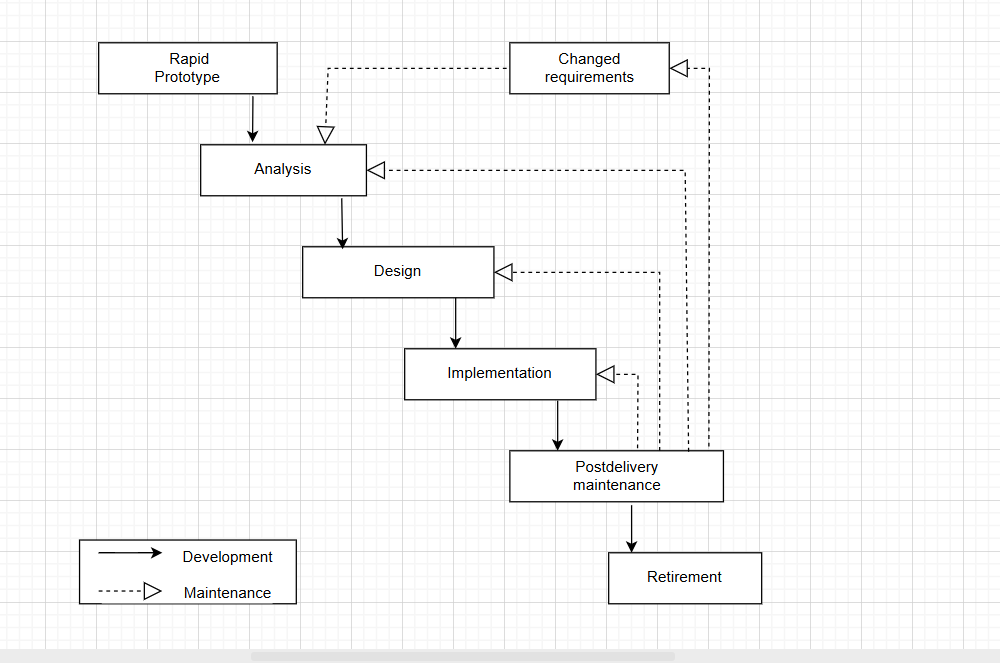
\includegraphics[width=15cm, height=7cm]{chapters/Prototype new.png}
    \caption{Selection Of Life Cycle Model (Prototype Model}
    
    %\vspace{-0.3cm}
\end{figure}

Waterfall Model  is best suited model for this project:
\begin{enumerate}
    \item 	The system requirements are clear and well-documented..
    \item 	The development process is straightforward, with distinct phases of analysis, design, implementation, testing, and deployment.

   \item Limited user participation is required during early stages, making it ideal for academic projects.
 
   \item Ensures timely completion of each phase before moving to the next.

\end{enumerate}


\section{Organization of Report}

The organization of the report is structured as follows:

\begin{itemize}

\item \textbf{CHAPTER 1} \\
Titled as \textbf{Introduction}, this chapter describes the background of the project, problem definition, scope and objectives, and the overall structure of the report.

\item \textbf{CHAPTER 2} \\
Titled as \textbf{Planning}, this chapter includes feasibility study, risk analysis, project scheduling, effort estimation, and cost estimation.

\item \textbf{CHAPTER 3} \\
Titled as \textbf{Analysis}, this chapter explains requirement collection and identification, hardware and software requirements, functional and non-functional requirements.

\item \textbf{CHAPTER 4} \\
Titled as \textbf{Design}, this chapter presents system architecture, data flow diagrams, database design, and UML diagrams.

\item \textbf{CHAPTER 5} \\
Titled as \textbf{Coding/Implementation}, this chapter describes the algorithms, development tools, technologies used, and different modules implemented in the system.

\item \textbf{CHAPTER 6} \\
Titled as \textbf{Testing}, this chapter includes testing methodologies such as black box and white box testing, manual and automated testing, and test case identification and execution.

\item \textbf{CHAPTER 7} \\
Titled as \textbf{Results and Discussion}, this chapter presents the output of the system, performance analysis, and discussion of the results obtained.

\item \textbf{CHAPTER 8} \\
Titled as \textbf{Conclusion and Future Work}, this chapter summarizes the overall project outcomes and suggests possible future enhancements.

\end{itemize}





\end{itemize}

\section{Summary}
 In this Chapter, Introduction is presented. In the next Chapter, Project Planning And Management is discussed.





\chapter{Project Planning and Management}\index{Project Planning and Management}

\justifying 
Project planning is a procedural step in project management. It is the practice of initiating,
planning, executing, controlling, and closing the work team to achieve specific goals. Project
planning and management are important because it ensures that the right people do the right
things, at the right time. It also ensures the proper project life cycle.

The organization of the Chapter is as follows . The Section 2.1 shows the Feasibility
Study of the project. Risk Analysis of the project is represented in Section 2.2. Project
Scheduling is described in Section 2.3. The Section 2.4  describes the effort allocation, Cost Estimation given in Section 2.5 respectively. Summary is mentioned in Section 2.6.


\section{Feasibility Study}

A feasibility study is an important step in software development that evaluates the practicality and success potential of a project. In this project, namely the Virtual Lab Assistant for DBMS practical examination, the feasibility study helps in identifying whether the system can be developed and implemented effectively.

The study focuses on analyzing different aspects such as technical feasibility, operational feasibility, and economic feasibility. It helps in understanding the strengths, weaknesses, opportunities, and possible risks associated with the system. This ensures that the project is realistic and achievable within the available resources and time.

The system is designed as a web-based platform using modern technologies such as Firebase, HTML, CSS, and JavaScript. It provides features like student authentication, practical exam execution, performance tracking, and secure session handling. The feasibility study evaluates whether these features can be efficiently developed and maintained.



\subsection{Technical Feasibility}
The technical feasibility of the proposed VR-Lab Assistant system is evaluated based on the system requirements and the technologies used for development. The objective is to determine whether the available technical resources are sufficient to successfully design and implement the system.

The project is developed using HTML, CSS, and JavaScript for the frontend, along with Firebase (Authentication and Firestore Database) for backend services. Firebase provides real-time database support, secure authentication, and cloud-based storage, eliminating the need for complex server-side setup


\subsection{Operational Feasibility}

Operational feasibility evaluates how effectively the VR-Lab Assistant system will function within the existing educational environment.

The system is designed to assist students in performing virtual practicals and conducting online examinations in a structured and interactive way. It provides features such as:
\begin{enumerate}
\item Student login and authentication
\item Admin control panel
\item Practical execution with real-time query evaluation
\item Performance tracking and progress visualization
\end{enumerate}
\subsection{Economic Feasibility}
Economic feasibility determines whether the project is cost-effective and beneficial compared to traditional methods.

The VR-Lab Assistant system is highly economical as it uses free or low-cost technologies such as Firebase and web-based tools. There is no need for expensive hardware, licensed software, or dedicated servers.



\section{Risk Analysis}
• The Virtual Lab Assistant project faces potential risks in technical, security, and
operational areas that could affect its smooth execution and reliability. Key concerns
include dependency on APIs, database performance, system security, and user
adoption. However, with planned mitigation strategies like fallback systems, testing,
monitoring, and strict schedule adherence, these risks can be effectively managed to
ensure stable and secure project delivery.

\item  Technical Risks


• Possible query evaluation inaccuracies affecting grading credibility.

• Firebase scaling or outage risks causing downtime or performance issues.

• Security and Integrity Risks

• Attempts to bypass exam security features like tab restriction or copy-paste blocking.

• Potential data breaches exposing student or exam information.

• Operational and Usability Risks

• Resistance to platform adoption by faculty or students.


• Delays in project completion due to the tight four-week schedule. 

\item 
\item 
\item 

\section{Project Scheduling}
Project scheduling is an essential part of project planning that defines the timeline and sequence of activities required for successful completion of the project. It helps in organizing tasks, allocating time efficiently, and ensuring that the project progresses in a structured manner. A well-defined schedule allows developers to track progress, identify delays, and manage resources effectively.

 
\raggedright 
\subsection{Week-by-Week Breakdown}

\begin{itemize}

\item \textbf{Week 1:} Focuses primarily on Planning / Requirements and initiating the Analysis \& Design phase.

\item \textbf{Week 2:} The Analysis \& Design phase continues, and the bulk of the Implementation / Development work begins.

\item \textbf{Week 3:} Is the most intensive week, featuring major activities in Implementation / Development, the commencement of Testing, and the start of Review / Evaluation.

\item \textbf{Week 4:} Concludes the project with the final activities for Implementation / Development and Testing. It also includes the continuation of Review / Evaluation and the final stage of Deployment / Integration.

\end{itemize}
\end{figure}
\newpage

\justifying 
\section{Effort Allocation}
Effort allocation refers to the amount of time a task should take from an assignee’s day. A project involves teamwork, where development is the result of combined efforts from the team. The project is divided into modules, with a number of modules allocated to team members. After completion of each module, it will be linked to other modules to form a complete project. Effort allocation should serve as a guideline only. The characteristics of each project will determine the distribution of effort. The effort allocation table for the proposed system is shown in the following table. Table 2.1 shows Effort Allocation for Project.
%\centering

%\text{Table 2.2 : Effort Allocation }\vspace{0.5cm}
%\index{ Effort Allocation for Project}
\begin{table}[H]
  %\centering
  % Your table content here
  \caption{Effort Allocation for Project}\index{ Effort Allocation for Project}
\end{table}


   \begin{tabular}{|p{0.6cm}|p{6.7cm}|p{1.8 cm}|p{1.9 cm}|p{1.8cm}|p{1.8cm}|}
       
        \hline
        Sr. no & Module & Pradnya & Chhayshree & Gauri & Saniya \\ \hline
        1 & Gathering Of Information & \checkmark& & \checkmark & \\ \hline
        2 & Planing/Requirement Analysis & \checkmark  & \checkmark &  & \checkmark \\ \hline
        3 & Selection of life cycle &  & \checkmark & \checkmark & \checkmark \\ \hline
        4 & Planning and management & \checkmark & \checkmark &  & \\ \hline
        5 & Analysis \& Design UML  & \checkmark & \checkmark & \checkmark & \checkmark \\ \hline
        
   \end{tabular}]

%\begin{table}[H]
%  \centering
  % Your table content here
 % \caption{Effort Allocation for Project}
%\end{table}

\newline
\section{Cost Estimation}


The Virtual Lab Assistant project is highly cost-effective, leveraging free and freemium tools to minimize expenses. With HTML, CSS, and JavaScript for the frontend and Firebase (using Google’s free Spark Plan) for the backend, initial development costs remain minimal. The only significant variable expense arises from the OpenAI API, which operates on a pay-as-you-go model based on hint usage. Overall, the project maintains a low initial cost structure, with expenses scaling only as user activity increases.

The cost estimation model used in this project follows a \textbf{Zero-Based Budgeting approach} combined with a \textbf{Lean/Startup Cost Structure}. In this approach, development begins with an estimated cost of ₹0 for most components such as frontend development, backend development, database, testing, and maintenance, and expenses are added only where absolutely necessary (such as domain name, contingency, and API usage).

\subsubsection{Key Cost Factors}

\begin{itemize}

\item \textbf{Frontend:} Built using free technologies such as HTML, CSS, and JavaScript, resulting in no licensing cost.

\item \textbf{Backend \& Database:} Hosted on Firebase Freemium (Spark Plan), where costs scale based on usage.


\item \textbf{Operational Costs:} Includes Firebase reads/writes, hosting, and storage, all of which are usage-dependent.

\item \textbf{Cost Optimization:} A preloaded hints database is used as an alternative to reduce dependency on the OpenAI API and minimize costs.

\end{itemize}

The project provides a low-cost and scalable solution with minimal upfront investment and manageable variable expenses, making it suitable for educational environments.

\newline


\section{Summary}
Project Scheduling and Effort Allocation
The project follows an intensive four-week schedule to manage the workload from conception
to deployment. Effort allocation is distributed across six phases: 





\chapter{Analysis}\index{Analysis}
\justifying 
The Chapter presents a detailed examination of the Virtual Lab Assistant project.
Analysis simplifies the project by dividing it into different parts, which is a crucial process for effective software development.
\item The organization of this Chapter is as follows:
Section 3.1 focuses on Requirement Collection and Identification.
The Software Requirement Specification (SRS) is presented in Section 3.2.
Section 3.3 summarizes the entire Chapter.


\section{Requirement Collection and Identification}
Requirement Collection and Identification is a critical step in the development of the Virtual Lab Assistant system. It involves gathering, analyzing, and defining the needs of users, including students and administrators.

The requirements were identified through observation of existing practical examination systems and understanding the challenges faced during manual practical sessions. Key requirements include user authentication, practical execution, real-time query evaluation, performance tracking, and admin control functionalities.


\section{Software Requirement Specification (SRS)}
The Software Requirement Specification (SRS) for the Virtual Lab Assistant defines its functionality, user roles, and environmental needs. It ensures a clear understanding between developers, faculty, and students, minimizing ambiguity during development.
This section outlines the functional, non-functional, and external requirements essential to the project.
\subsection{Product Features}
- User Management: Registration and login system for students using PRN numbers, and secure login for admin users.  

\item- Subject & Practical Management:
: Supports multiple subjects (DBMS, C, C++, Python). Each subject contains 10 practicals with 10 related questions 
\item - Exam Controls: admin can see the progress of students and modify questions per subject  Students can only attempt practicals on their scheduled date.

\item- Question Handling:: Each question includes an example, a hint, and code/SQL input support  

\item- Evaluate & Submit Feature: Students can simulate “evaluate” operations and submit their solutions for evaluation

\item- Timer & Attempt Control: Each exam runs under a timer (30 minutes) with automatic submission on timeout. Login attempts are limited to prevent misuse
\item- Feedback & Help Section: Students can send feedback and contact administrators directly from the platform.
\item- Performance Tracking: Admin can monitor completion percentages of subjects and practicals through progress indicators.

\subsection{Operating Environment}
Software and hardware environments, referred to as the operating environment for the project, are outlined as follows:


\begin{enumerate}
  \item	Operating Environment:
The Virtual Lab Assistant is a web-based platform accessible from any modern browser such as Google Chrome, Firefox, or Edge.
It can be hosted on any web server supporting HTML, CSS, and JavaScript for the frontend and future integration with PHP or Node.js for the backend.
Secure communication (HTTPS) ensures safe data transfer.


 
  \item	Hardware Environment:
The system requires only basic hardware — desktop, laptop, or tablet with an internet connection.
A server with at least 4 GB RAM and SSD storage is recommended for efficient performance and scalability.




\end{enumerate}
\newpage
\subsection{Assumptions} 
The following assumptions are made during the development and usage of the Virtual Lab Assistant:

\begin{itemize}

    \item	Users (students and administrators) will have access to stable internet connectivity.
    \item	Students have basic computer and internet literacy.
    \item	Admin users will maintain the correctness of practical questions 
    \item	All users will operate the system through authorized login credentials.
    \item	The server environment will support standard web technologies and ensure data backup.
    \item	The system will be scalable to accommodate an increasing number of students and subjects.

 
\end{itemize}

\subsection{ Functional Requirements}
The Virtual Lab Assistant system includes the following functional requirements:
\subsubsection{\textbf{System}}
\begin{enumerate}
  

   \item 	Student Registration and Login:
Students can register with PRN and password and log in securely.
    \item	Practical Execution:
Students can start subject-specific practicals, compile code, get hints, and submit answers.
   
    \item	Question Management:
Admin can modify or add new questions per subject and practical.
    \item	Performance Monitoring:
The system shows progress completion bars for each subject’s practicals.
    \item	Feedback Submission:
Students can send feedback or queries to the admin using a contact form.
    \item	Session Management:
Each login is tracked, and excessive login attempts result in account lockout.

%\end{enumerate}
%\subsubsection{\textbf{User}}
%\begin{enumerate}
%    \item Give overall information to the system. 
 %    \item  View diet plan, exercise, nutritions according to BMI calculation. 
  %  \item Set their daily routine
%\end{enumerate}
\newpage
\subsection{Non Functional Requirements}
Non-functional requirements define the quality attributes of the Virtual Lab Assistant rather than the specific behaviors.
While functional requirements determine what the system should do, non-functional requirements specify how well it should perform under various conditions.
\begin{enumerate}
    \item Performance Requirement:- The system should respond within 2 seconds for major actions such as login, compile, or submit.

   \item  Availability:- The web application should be accessible 24/7, ensuring minimal downtime.
   
  \item Usability:- The interface should be user-friendly, easy to navigate, and consistent across devices.

   \item Consistency:-The interface should be user-friendly, easy to navigate, and consistent across devices.
   
  \item Reusability:- Question templates and student evaluation components can be reused for multiple subjects or academic years.

\end{enumerate} 

\section {External Interfaces}
Some External interfaces are as follows:
\begin{enumerate}
    \item User Interface
    \item Hardware Interface
    \item Software Interface

 
\subsection{User Interface}
  The proposed system has several options for users to interact with. Following are the user interfaces available:

    •	Web Application:
Provides a graphical interface for both students and administrators. Students can log in, attempt practicals, and view progress.

•	Admin Dashboard:
Allows administrators to set dates, manage subjects, and update questions.

   

   

\subsection{Hardware Interface}
  •	Compatible with desktops, laptops, and tablets.

•	Optional integration for printing student performance reports.


\subsection{Software Interface}
 •	The application supports integration with backend databases (Firebase).

•	Can connect with cloud-based storage or external APIs for future expansion.
.

\subsection{Communication Interface}
•	Uses HTTP/HTTPS for secure data transfer between the client and server.

•	Can integrate with email or SMS APIs for notifications in future updates.



\end{enumerate}






\section{Summary}
This Chapter provided a comprehensive analysis of the Virtual Lab Assistant project.
It covered requirement collection, software specifications, and external interfaces.
The study identified key functional and non-functional requirements, ensuring that the system meets academic and operational needs.
The Virtual Lab Assistant offers an innovative, scalable, and secure way to conduct online practicals efficiently while supporting both students and faculty through a seamless digital platform.


\chapter{Design}\index{Design}
\justifying 
System design provides the understanding and procedural details necessary for implementing
the system.Design builds coherent, well planned representations of programs that concentrate
on the interrelationships of parts at the higher level and the logical operations involved at the
lower levels. Software design is the first of the three technical activities designs, coding and test
which are required to build and verify the software

The organization of the Chapter is as follows.Section 4.1 describes the system architecture of the Virtual Lab Assistant. The Data Flow Diagrams (DFDs)
of the project are presented in Section 4.2. Section 4.3 covers various UML diagrams
including Use Case Diagram, Sequence Diagram, Collaboration Diagram, Class Dia-
gram, Component Diagram, and Deployment Diagram, the summary of the
chapter is provided in Section 4.4.

\section{System Architecture}
System architecture refers to the high-level design and structure of a complex system, outlining
its components, interactions, and organization to achieve specific objectives. It defines the
system’s key building blocks, functions, and how they communicate with each other and
external entities. A well-defined system architecture provides a blueprint for system
development, enabling efficient implementation, scalability, and maintenance while ensuring
that the system meets its intended goals and requirements. It often includes various
architectural layers, modules, interfaces, and data flows, which collectively shape the system’s
behavior and performance.

\begin{figure}[H]
    %\begin{center}
    \centering
    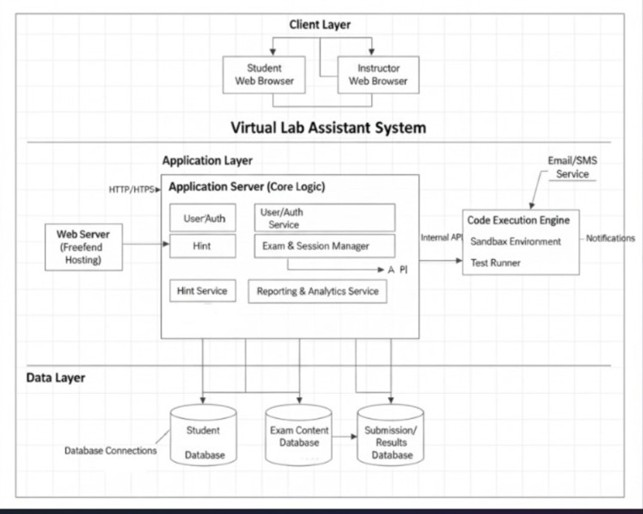
\includegraphics[width=15cm, height=12cm]{chapters/sysarchi.jpg}
    \caption{System Architecture}
    
    %\vspace{-0.3cm}
\end{figure}


\section{Data Flow Diagram}
A Data Flow Diagram (DFD) is a graphical representation used in system analysis and design to illustrate the flow of data within a system. It visually depicts processes, data stores, data flows, and external entities, providing a clear and concise overview of how data moves through a system and how different components interact. DFDs are instrumental in understanding, designing, and documenting information systems and processes.


\subsection{Level 0 DFD}
Level 0 Data Flow Diagram (DFD) is highest-level view of system’s data flow. It provides a simplified, bird’s-eye perspective, showing major processes or functions within system, external entities interacting with it, and primary data flows between them. Diagram serves as an initial overview of system architecture and helps stakeholders grasp system scope and boundaries.The Figure 4.2 shows Level 0 DFD Diagram.
\begin{figure}[H]
    %\begin{center}
    \centering
    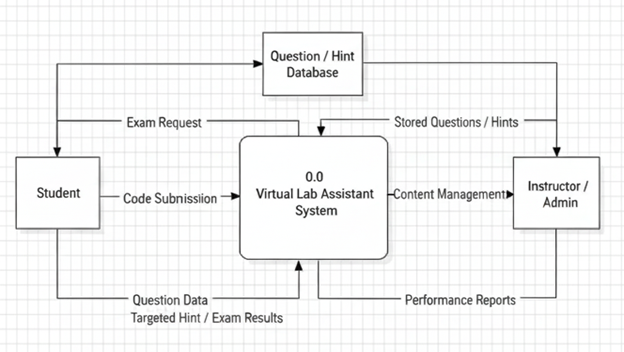
\includegraphics[width=15cm, height=5cm]{chapters/odfd.png}
 \caption{Level 0 DFD Diagram}\label{Fig:my_label}
    %\vspace{-0.3cm}

  \end{figure}
\subsection{Level 1 DFD}
A Level 1 Data Flow Diagram (DFD) is a more detailed representation that expands on the processes identified in the Level 0 DFD. It breaks down these processes into sub-processes or functions and provides a closer look at how data flows between them. Level 1 DFDs are used to gain a deeper understanding of the system's internal operations and data transformations, making them valuable for system analysis, design, and documentation. The Figure 4.3 shows Level 1 DFD Diagram.
\begin{figure}[H]
    %\begin{center}
    \centering
    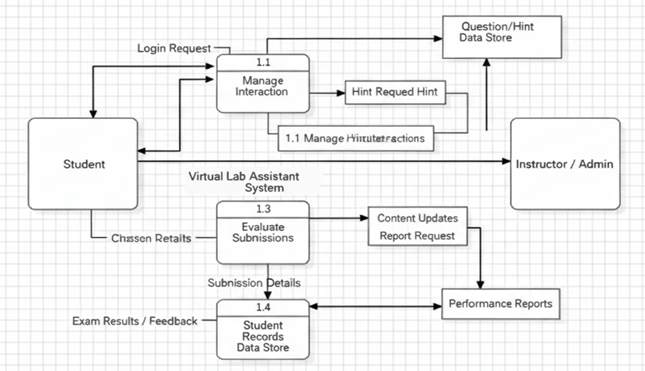
\includegraphics[width=15cm, height=8cm]{chapters/1dfd.png}
    \caption{Level 1 DFD Diagram}\label{Fig:my_label}
      
      \centering
\end{figure}


         \newpage  
\subsection{Level 2 DFD}
A Level 2 DFD is a detailed breakdown of processes from a Level 1 DFD, showing specific sub-processes, finer data flows, and detailed interactions with data stores and entities. It provides a deeper insight into how data is processed and managed within critical system components, aiding in precise system analysis and design. The Figure 4.4 shows Level 2 DFD Diagram
\begin{figure}[H]
    %\begin{center}
    \centering
    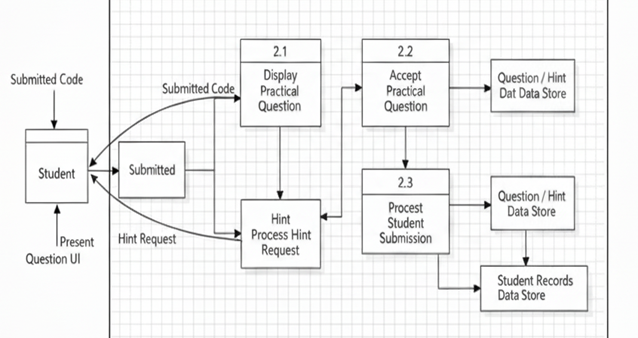
\includegraphics[width=15cm, height=12cm]{chapters/2dfd.png}
  \caption{Level 2 DFD Diagram}\label{Fig:my_label}
    %\vspace{-0.3cm}
\end{figure}

\newpage

\section{UML Diagrams}
Unified Modeling Language (UML) diagrams are a standardized set of visual representations used in software engineering and system design to model, document, and communicate complex systems and their components. UML diagrams include various types, such as Use Case diagrams for capturing system interactions, Class diagrams for depicting the structure and relationships of system objects, Sequence diagrams to show the sequence of interactions, Collaboration diagrams for illustrating collaborations among objects, and many more. These diagrams serve as powerful tools for software developers, designers, and stakeholders to visualize, analyze, and communicate the architecture, behavior, and interactions of software systems, enhancing the understanding and effectiveness of the design and development processes.



\subsection{Use Case Diagram}

Use case diagram shows the interaction between Use case which represents system functionality and actor which represent the people or system.The Figure 4.5 shows Use Case Diagram.

\begin{figure}[H]
    %\begin{center}
    \centering
    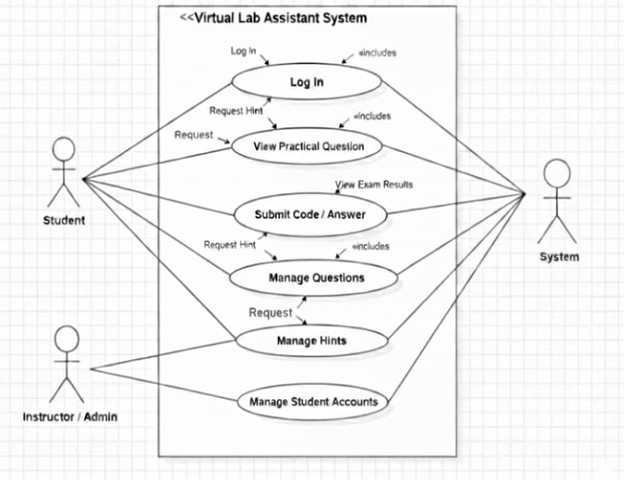
\includegraphics[width=13cm, height=15cm]{chapters/usecase.jpg}
    \caption{Use Case Diagram}\label{Fig:my_label}
    %\vspace{-0.3cm}
\end{figure}
\newpage

\subsection{Sequence Diagram}
The sequence diagram shows the flow of functionality through UseCase.A sequence diagram is a type of interaction diagram because it describes how and in what order a group of objects works together.These diagrams are used by software developers and business professionals to understand requirements for a new system or to document an existing process.The Figure 4.6 shows Sequence Diagram.


\begin{figure}[H]
    %\begin{center}
    \centering
    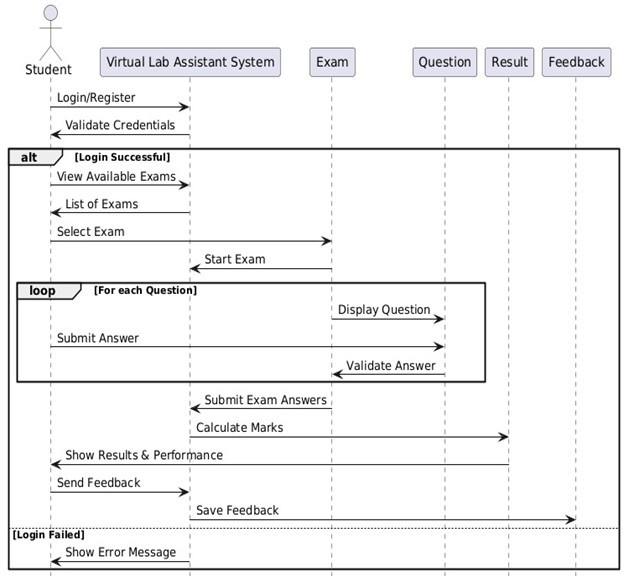
\includegraphics[width=15cm, height=13cm]{chapters/seq.jpg}
    \caption{Sequence Diagram }\label{Fig:my_label}
   % \caption{Sequence Diagram for Ideal Diet UseCase of Diet Planner Using BMI Calculation}
    %\vspace{-0.3cm}
\end{figure}
  % Figure :Sequence diagram for Admission Confirm use case of CAMS. 
\newpage




\subsection{Class Diagram}
The class diagram is the main building block of object- oriented modeling.It is used for general conceptual modeling of the structure of the application, and for detailed modeling translating the models into programming code.Class diagrams can also be used for data modeling.The Figure 4.7 shows Class Diagram.
\vspace{2cm}


\begin{figure}[H]
    %\begin{center}
    \centering
    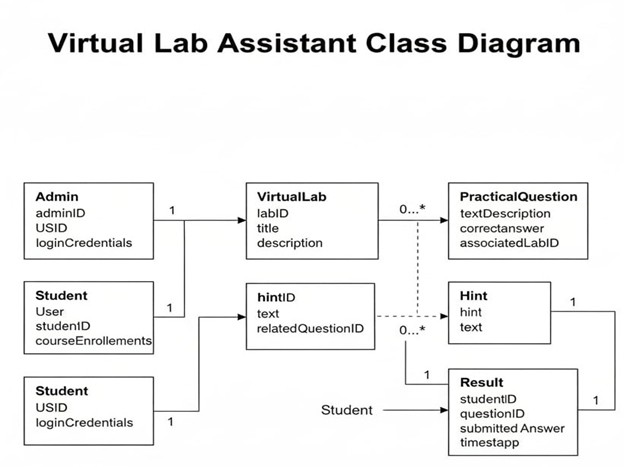
\includegraphics[width=15cm]{chapters/classi.jpg}
     \caption{Class Diagram}\label{Fig:my_label}
  %  \caption{Class Diagram for Diet Planner using BMI calculation}
    %\vspace{-0.3cm}
\end{figure}
\newpage




\subsection{Component Diagram}
A component diagram, also known as a UML component diagram, describes the organization and wiring of the physical components in a system.Component diagrams are often drawn to help model implementation details and double check that every aspect of the system’s required functions covered by planned development.The Figure 4.8 shows Component Diagram.


\begin{figure}[H]
    %\begin{center}
    \centering
    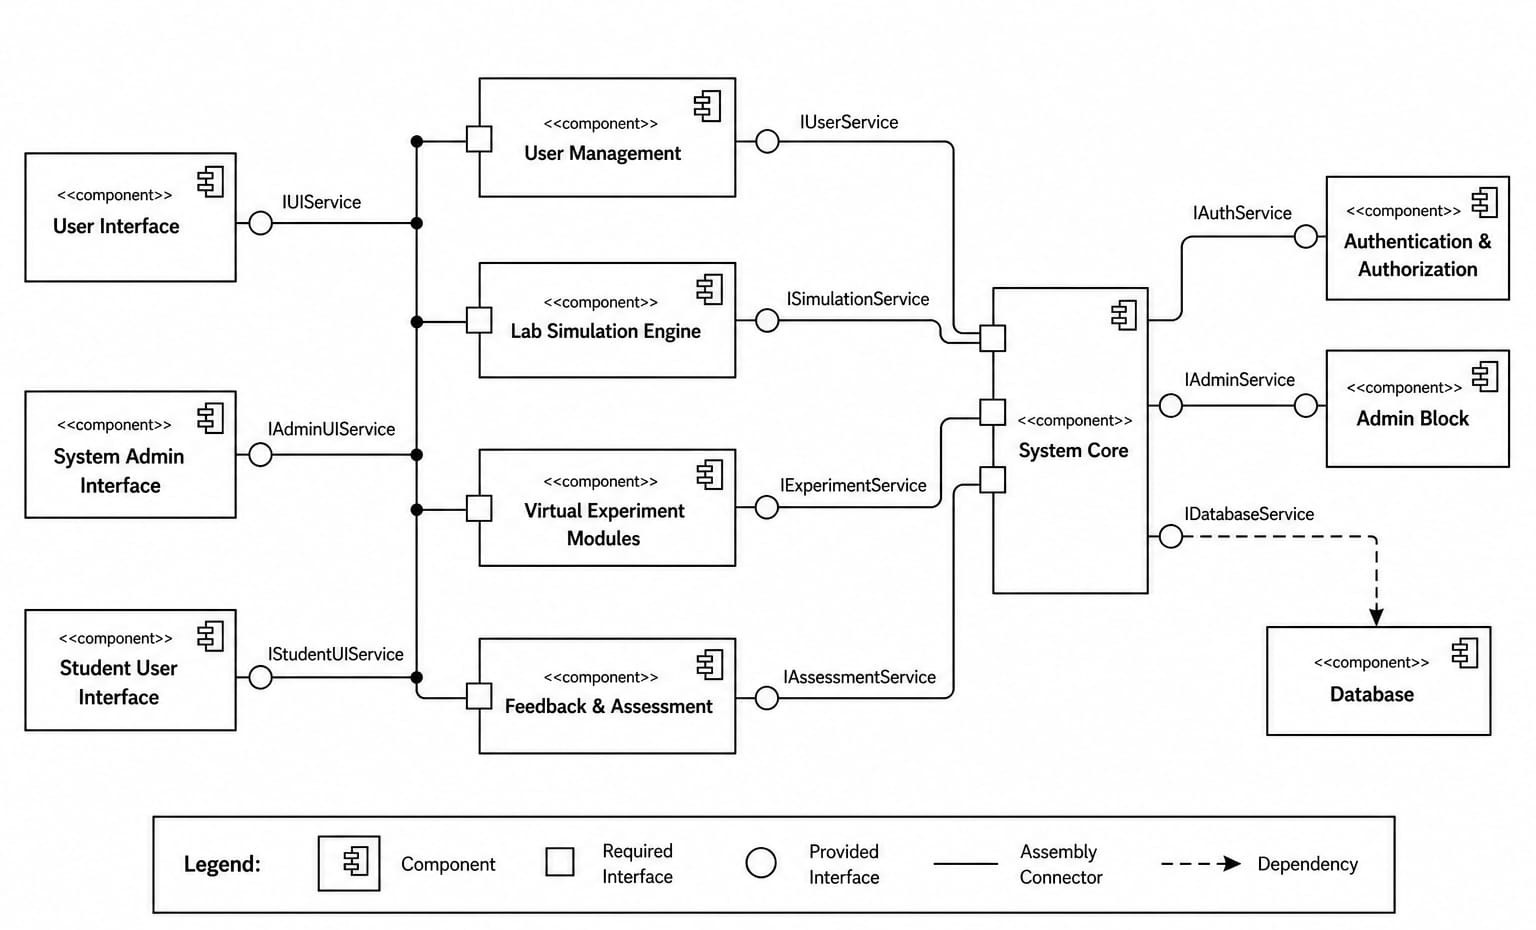
\includegraphics[width=15cm]{chapters/compo.jpeg}
      \caption{Component Diagram}\label{Fig:my_label}
   % \caption{Component Diagram For Diet Planner using BMI Calculation}
    %\vspace{-0.3cm}
\end{figure}
\newpage

\subsection{Deployment Diagram}
A deployment diagram is a UML diagram type that shows the execution architecture of a system, including nodes such as hardware or software execution environments, and the middle ware connecting them.Deployment diagrams are typically used to visualize the physical hardware and software of a system.The Figure 4.9 shows Deployment Diagram.


\begin{figure}[H]
    %\begin{center}
    \centering
    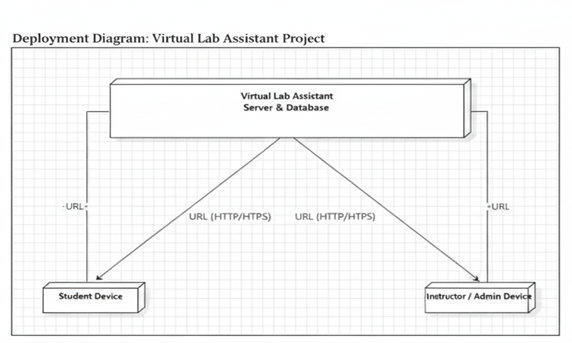
\includegraphics[width=15cm]{chapters/dep.png}
    \caption{Deployment Diagram}\label{Fig:my_label}
   % \caption{Deployment Diagram for Diet Planner using BMI Calculation}
    %\vspace{-0.3cm}
\end{figure}
\section{Summary}
n this Chapter, Design is presented. In the next Chapter, the Coding and Implementation
will be discussed .




\chapter{Coding / Implementation}

Coding and implementation provide the practical realization of the system by transforming the design into an executable application.

The implementation of the Virtual Lab Assistant is carried out using modern web technologies such as HTML, CSS, and JavaScript for the frontend, and Firebase for backend services including authentication, database management, and hosting. The system is developed in a modular manner to ensure scalability, maintainability, and ease of updates.


The organization of this chapter is as follows. Section 5.1 describes the algorithms
and step-by-step procedures used in the system. the software
and hardware requirements needed for development are explained in Section 5.2. Section 5.3 presents the various
modules of the project along with their implementation details, a summary of the chapter provided in Section 5.4.


\section{Algorithm / Steps}
The following steps describe the working process of the Virtual Lab Assistant system. 
It explains how the system handles user authentication, exam flow, query evaluation, and result storage.

\begin{enumerate}

\item Display login/registration page.
\item User enters PRN and password.
\item Authenticate user using Firebase Authentication.
\item Check session control from database.
\item If system is free, allow login; otherwise restrict access.
\item Display list of practicals.
\item User selects a practical.
\item Display questions related to selected practical.
\item User writes SQL queries.
\item System validates queries and provides feedback.
\item Store results in Firestore database.
\item Update performance progress.
\item End session on logout or submission.
\end{enumerate}


\section{Software and Hardware Requirements}
This section describes the necessary software and hardware components required to run the Virtual Lab Assistant system efficiently.
\subsection{Software Requirements}
The following software technologies are used for development and execution of the system.
\begin{itemize}
\item Operating System: Windows/Linux
\item Frontend: HTML, CSS, JavaScript
\item Backend: Firebase (Authentication and Firestore)
\item Browser: Google Chrome / Edge
\item Database: Cloud Firestore
\end{itemize}

\subsection{Hardware Requirements}
The system requires basic hardware configuration to ensure smooth performance during execution.
\begin{itemize}
\item Processor: Intel i3 or above
\item RAM: Minimum 4 GB
\item Storage: 500 MB free space
\item Internet Connection: Required for Firebase services
\end{itemize}

\section{Modules in Project}
The project is divided into multiple modules, each responsible for handling specific functionalities of the system.
\subsection{Student Authentication Module}
Handles student registration and login using Firebase Authentication.


\subsection{Exam Module}
Displays practical list and manages question flow.

\subsection{Evaluation Module}
Validates SQL queries and provides instant feedback.

\subsection{Performance Tracking Module}
Tracks completed practicals and shows progress using a progress bar.

\subsection{Security Module}
Implements restrictions like disabling copy-paste, tab switching, and auto-submit.

\chapter{Testing}




In the Virtual Lab Assistant project, testing is performed at different levels to ensure that each module works properly both individually and when integrated with other modules. Various testing techniques such as Black Box Testing and White Box Testing are applied to validate system functionality and internal logic. Both manual and automated testing approaches are considered to ensure accuracy and efficiency.



The organization of this chapter is as follows. Section 6.1 describes Black Box and
White Box testing techniques. Manual and Automated testing
approaches are explained in Section 6.2. Section 6.3 presents test case identification and execution,  a summary of the chapter is described in Section 6.4

\section{Black Box Testing}
Black box testing is used to verify system functionality without knowing the internal code structure.
It focuses on validating outputs based on different input conditions.

\begin{itemize}
    \item Testing of system without knowledge of internal code structure.
    \item Focuses only on inputs and expected outputs.
    \item Used to validate functional requirements.
    \item Example: Checking login with valid and invalid credentials.
\end{itemize}

\section{White Box Testing}
White box testing is performed to analyze the internal working of the system and code logic.
It helps in verifying program flow, conditions, and execution paths.
\begin{itemize}
    \item Testing based on internal code logic and structure.
    \item Involves checking conditions, loops, and execution paths.
    \item Requires programming knowledge.
    \item Helps in improving code efficiency and coverage.
\end{itemize}

\section{Manual Testing}
Manual testing is carried out by testers without using any automation tools.
It is mainly used to check user interface and overall user experience.
\begin{itemize}
    \item Testing performed manually without automation tools.
    \item Tester executes test cases step by step.
    \item Useful for UI and user experience validation.
    \item Time-consuming but effective for small applications.
\end{itemize}

\section{Automated Testing}
Automated testing uses tools and scripts to perform testing tasks efficiently.
It improves speed, accuracy, and consistency in testing processes.
\begin{itemize}
    \item Testing performed using tools and scripts.
    \item Faster and more reliable than manual testing.
    \item Reduces human errors in repetitive tasks.
    \item Suitable for large-scale and continuous testing.
\end{itemize}

\section{Test Case Identification and Execution}
This process involves designing and executing test cases to ensure system correctness.
It helps in identifying errors by comparing expected and actual results.
\begin{itemize}
    \item Identify all functional modules of the system.
    \item Design test cases for valid and invalid inputs.
    \item Execute test cases and record outputs.
    \item Compare expected and actual results.
\end{itemize}
\subsection{Test Case Table}

\renewcommand{\arraystretch}{1.3}

\begin{table}[H]
\centering
\begin{tabular}{|c|c|c|c|c|c|}
\hline
Test ID & Input & Output & Expected Output & Actual Output & Result \\
\hline
TC01 & Valid Login & Success & Login Success & Login Success & Pass \\
\hline
TC02 & Wrong Password & Error & Error Message & Error Message & Pass \\
\hline
TC03 & Empty Fields & Warning & Warning Message & Warning Message & Pass \\
\hline
TC04 & Invalid PRN & Error & Invalid User & Invalid User & Pass \\
\hline
TC05 & Correct Query & Success & Query Executed & Query Executed & Pass \\
\hline
TC06 & Wrong Query & Error & Query Error & Query Error & Pass \\


\hline
TC08 & Timer Expired & Auto Submit & Exam Submitted & Exam Submitted & Pass \\
\hline
TC09 & Logout Action & Success & Logged Out & Logged Out & Pass \\

\hline
TC10 & Contact Form Submit & Success & Data Saved & Data Saved & Pass \\
\hline
\end{tabular}
\caption{Test Case Identification and Execution}
\end{table}

\chapter{Results and Discussion}

The obtained results indicate that the system operates efficiently and satisfies the expected project requirements. 
\subsection*{Results}

The Virtual Lab Assistant system was successfully developed and executed in a real-time environment. During testing, students were able to log in securely using PRN and password through Firebase Authentication and access the practical examination portal without difficulty. The system properly handled invalid login attempts and maintained secure session management.

During the practical examination process, students selected practicals and answered SQL-based questions using the integrated query editor. The compiler validated the syntax of queries and provided immediate feedback regarding correct or incorrect execution. The system successfully handled common SQL commands such as \texttt{SELECT}, \texttt{INSERT}, \texttt{UPDATE}, \texttt{DELETE}, and \texttt{ORDER BY}. 

The timer functionality worked accurately throughout the examination process and automatically submitted the practical when the examination time expired. Student performance and practical completion data were stored successfully in Firebase Firestore, and progress indicators dynamically displayed completion percentages.

From the administrator’s perspective, the system successfully displayed student records, submissions, and overall performance details. The admin panel helped in monitoring examination activities and managing the system efficiently.

\subsection*{Discussion}

The discussion of the results shows that the Virtual Lab Assistant system provides a reliable and user-friendly platform for conducting virtual practical examinations. The integration of Firebase Authentication and Firestore ensured smooth data handling and secure access control throughout the system.

The compiler module performed effectively for basic SQL query validation and helped students receive quick feedback during examinations. However, it was observed that some complex SQL queries were partially accepted due to limited logical query checking. This indicates that future improvements can be made by implementing advanced query evaluation techniques.

The automated timer and submission mechanism improved examination fairness and reduced manual supervision requirements. Additionally, the dynamic progress tracking system helped students monitor their practical completion status efficiently.

Overall, the system achieved the intended objectives and demonstrated the successful implementation of an automated virtual laboratory environment. The project proved to be efficient, organized, and suitable for conducting online practical examinations with real-time interaction and evaluation.

% ----------------------------------------------------

\chapter{Conclusion and Future Work}

The Virtual Lab Assistant system was successfully designed and implemented to provide a digital platform for conducting practical examinations and learning activities.

\section*{Conclusion}

The developed Virtual Lab Assistant successfully fulfills the objectives defined during the planning and analysis phases of the project. The system provides an effective solution for managing practical-based examinations in a digital environment. Features such as student authentication, practical execution, query compilation, AI-based hints, and performance tracking contribute to an improved learning experience.

The integration of Firebase ensures secure database management and smooth communication between different modules of the system. The project demonstrates that modern web technologies can be effectively used to create scalable, reliable, and user-friendly educational applications. Overall, the project offers a cost-effective and efficient solution for virtual practical laboratory management.

\section*{Future Work}

Although the current system performs efficiently, there is still scope for further enhancement and improvement. In the future, more advanced technologies and features can be integrated to improve system functionality and user experience. The implementation of AI-based automatic query checking and intelligent evaluation mechanisms can make the system more accurate and interactive.

The system can also be expanded to support multiple departments, subjects, and practical domains. Improvements in the user interface and graphical design can provide a better user experience. Additionally, the development of a dedicated mobile application can increase accessibility and allow students to use the platform more conveniently from different devices and locations.

% ----------------------------------------------------




\begin{thebibliography}{9}

\bibitem{ref1}
Soraya, G. V. (2022).
``Benefits and Challenges in the Implementation of Virtual Laboratories.''
\textit{Biochemistry and Molecular Biology Education}.

\bibitem{ref2}
Elmesery, M. (2025).
``Advantages and Disadvantages of Virtual Laboratory in Education.''
\textit{PraxiLabs}.

\bibitem{ref3}
De Jong, T., Linn, M. C., and Zacharia, Z. C. (2013).
``Physical and Virtual Laboratories in Science and Engineering Education.''
\textit{Science}, 340(6130), 305--308.

\bibitem{ref4}
Potkonjak, V., Gardner, M., Callaghan, V., Mattila, P., Guetl, C., Petrovi\'c, V. M., and Jovanovi\'c, K. (2016).
``Virtual Laboratories for Education in Science, Technology, and Engineering: A Review.''
\textit{Computers \& Education}, 95, 309--327.

\bibitem{ref5}
Heradio, R., de la Torre, L., Galan, D., Cabrerizo, F. J., Herrera-Viedma, E., and Dormido, S. (2016).
``Virtual and Remote Labs in Education: A Bibliometric Analysis.''
\textit{Computers \& Education}, 98, 14--38.

\end{thebibliography}

% ----------------------------------------------------


% --------------------------------------------------
\clearpage
\addcontentsline{toc}{chapter}{\indexname}
\printindex


\clearpage
\chapter*{Appendix}
\addcontentsline{toc}{chapter}{Appendix}

\appendix

% RESET ALIGNMENT (force normal layout)
\setlength{\leftskip}{0pt}
\setlength{\rightskip}{0pt}
\setlength{\parindent}{15pt}
\noindent
In this project, the appendix contains screenshots of the Virtual Lab Assistant system, including interfaces like the Home Page, Student Login Page, Admin Panel, and Contact Page. These visuals help in understanding the actual implementation and user interface of the system.
 \section*{Screenshots}

\begin{figure}[H]
    \centering
    
\includegraphics[width=16cm,height=250]{chapters/home.png}
    \caption{Home Page}
\end{figure}

\begin{figure}[H]
    \centering
    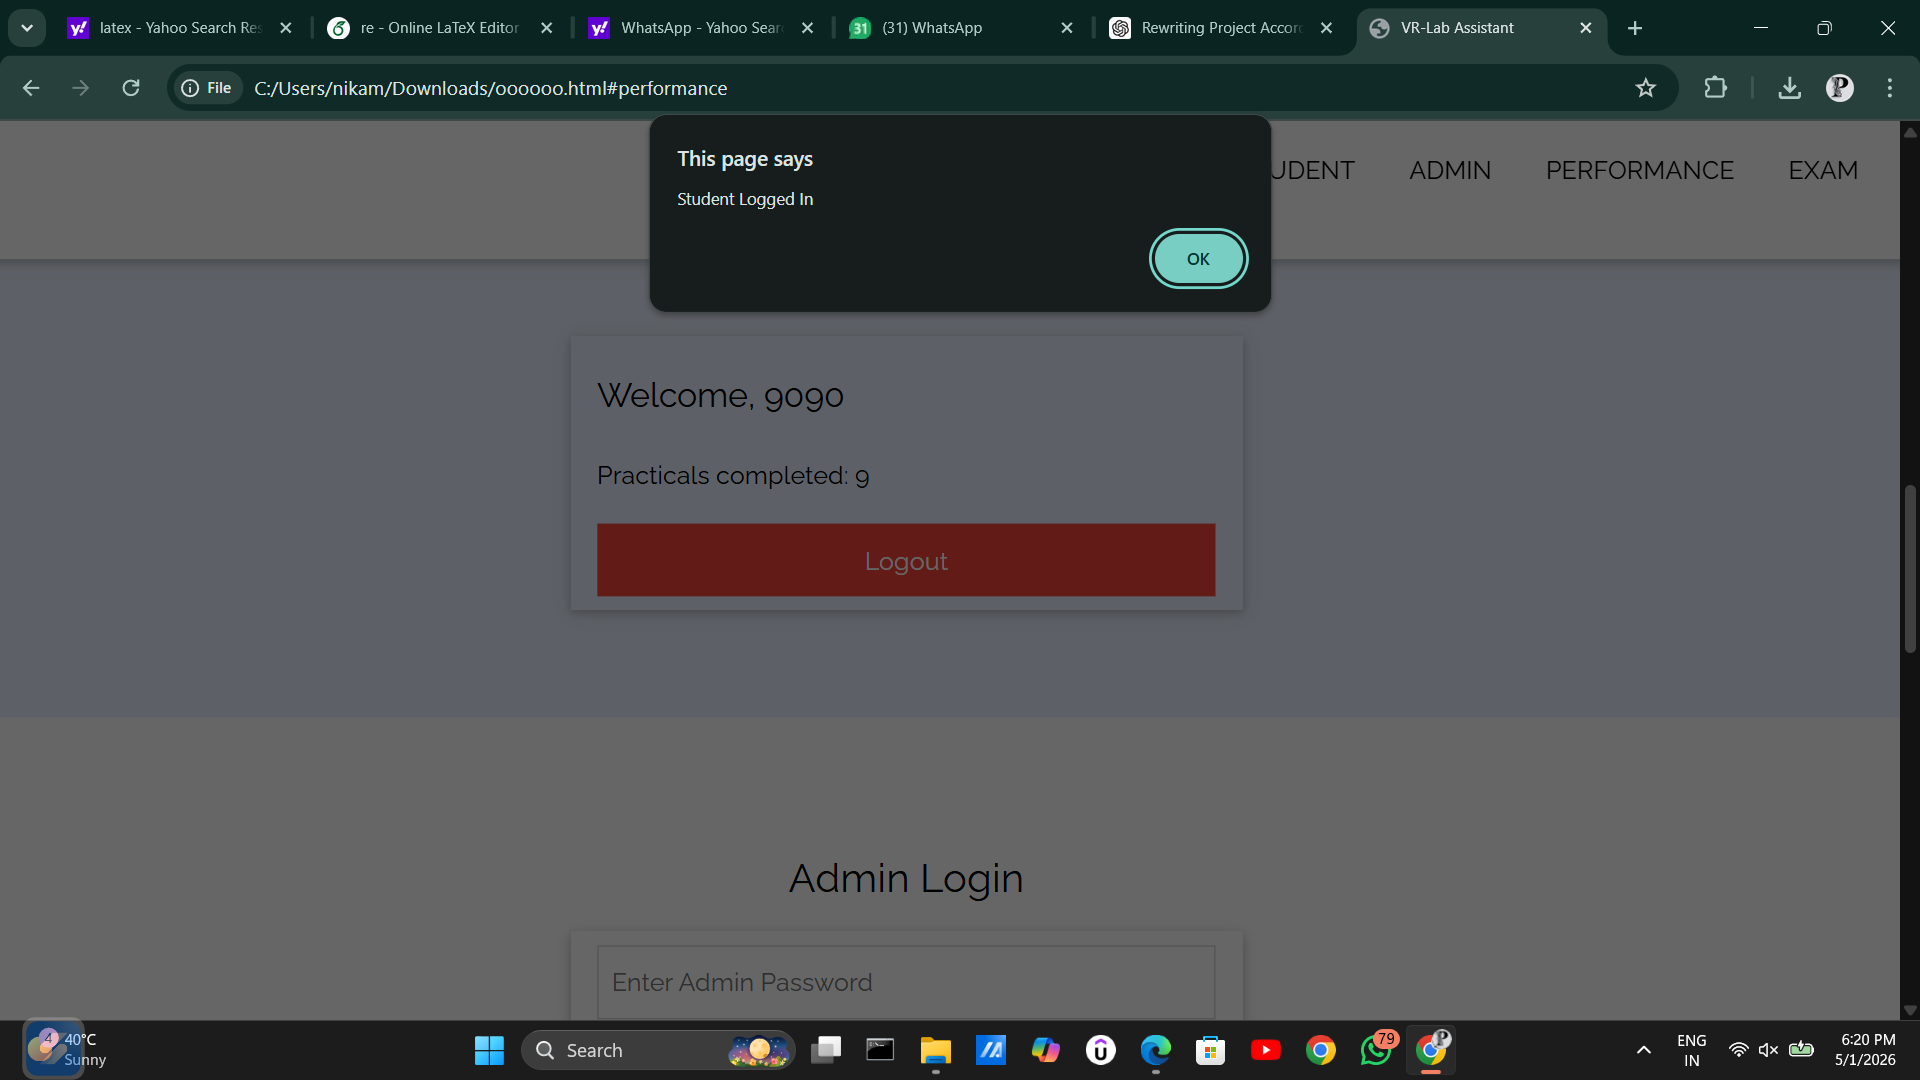
\includegraphics[width=16cm,height=250]{chapters/login.png}
    \caption{Student Login}
\end{figure}

\begin{figure}[H]
    \centering
    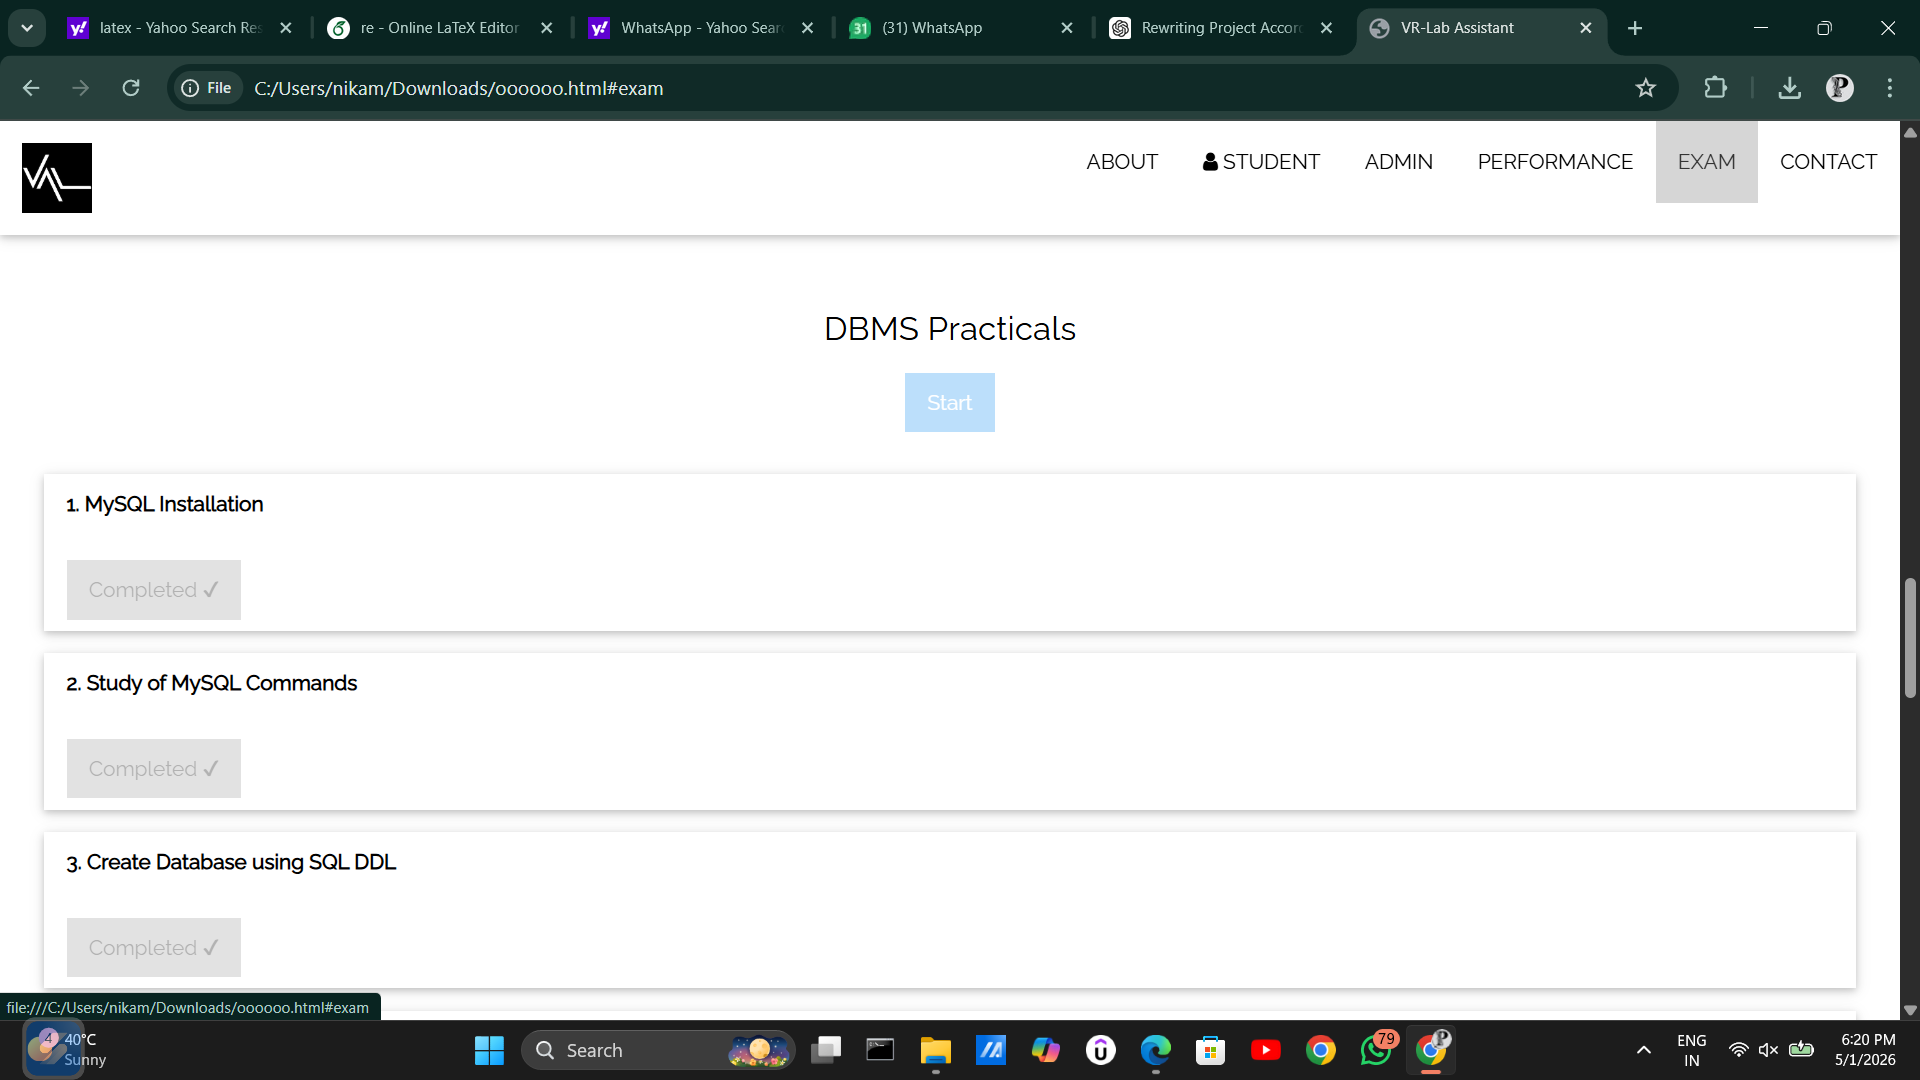
\includegraphics[width=16cm,height=300]{chapters/exampractical.png}
    \caption{Exam Practicals}
\end{figure}

 \begin{figure}[H]
    \centering
    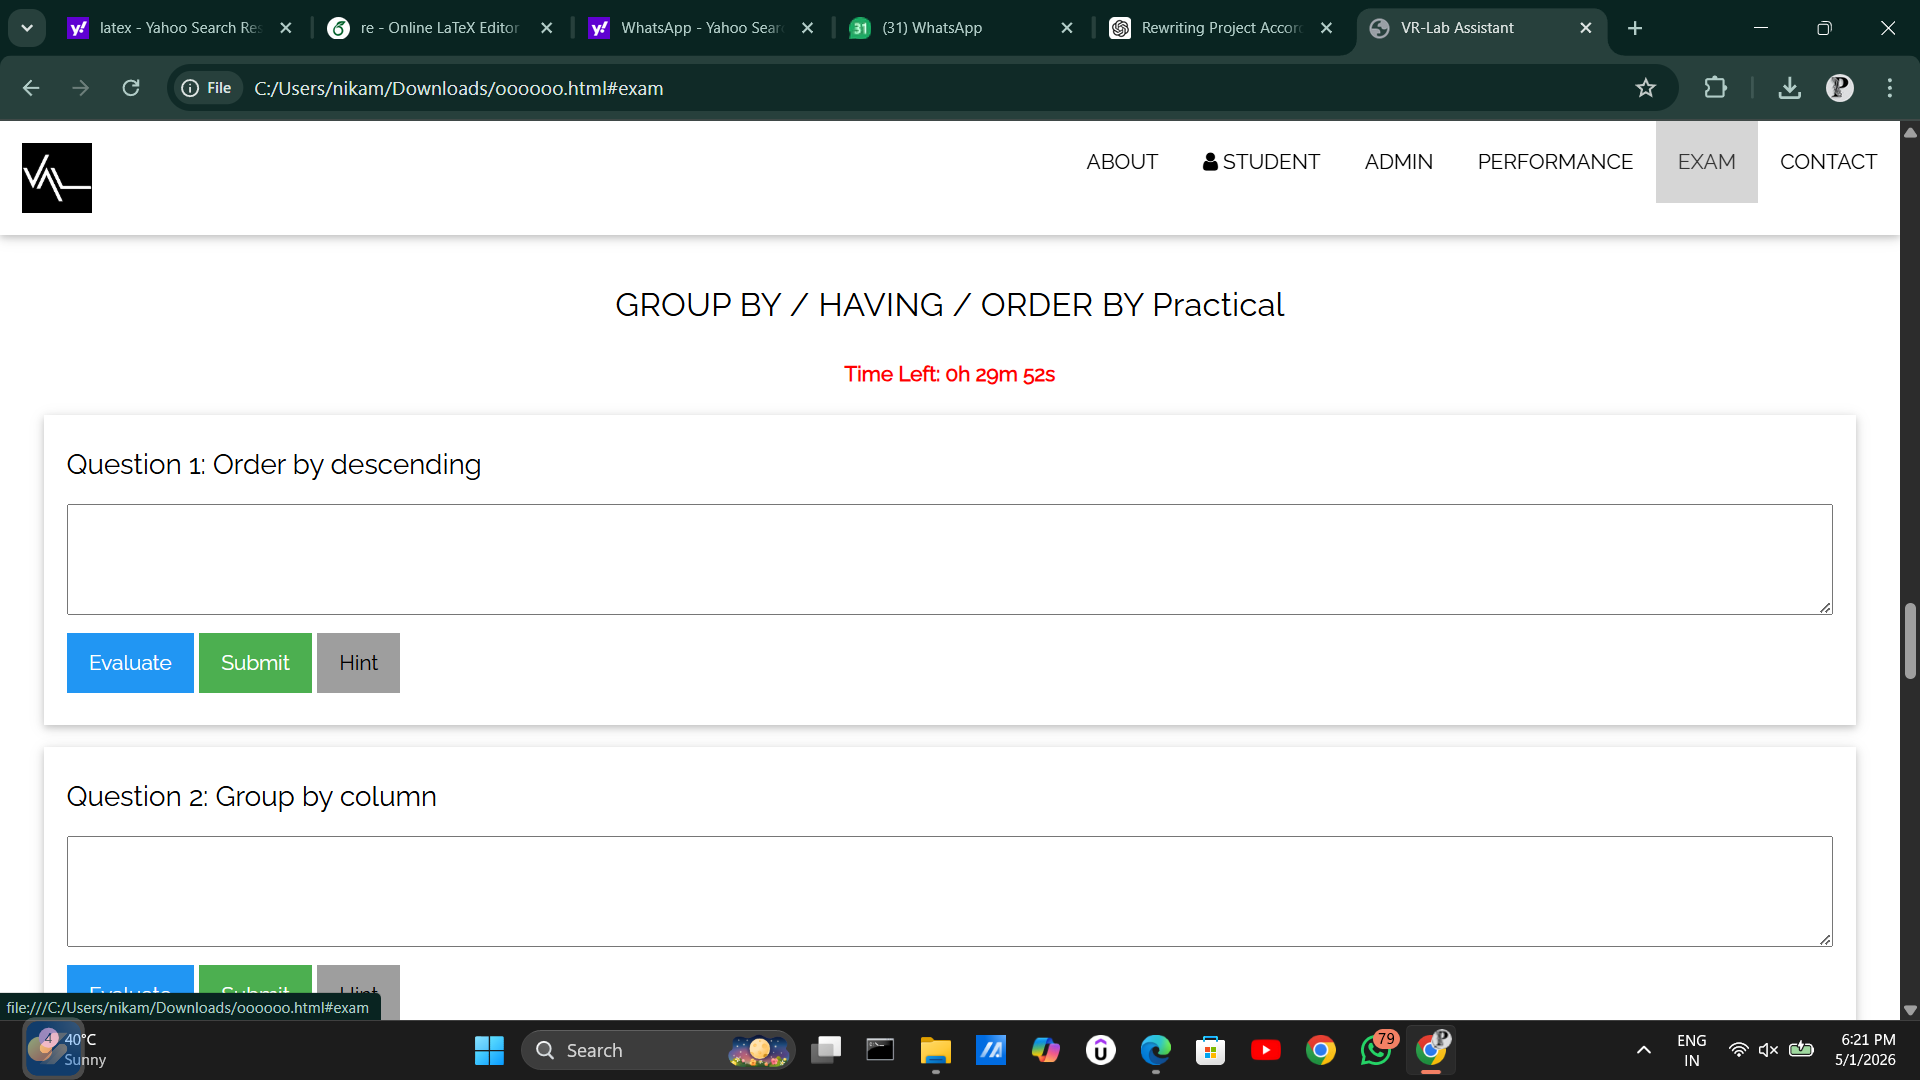
\includegraphics[width=16cm,height=300]{chapters/examstart.png}
    \caption{Exam Start}
\end{figure}

\begin{figure}[H]
    \centering
    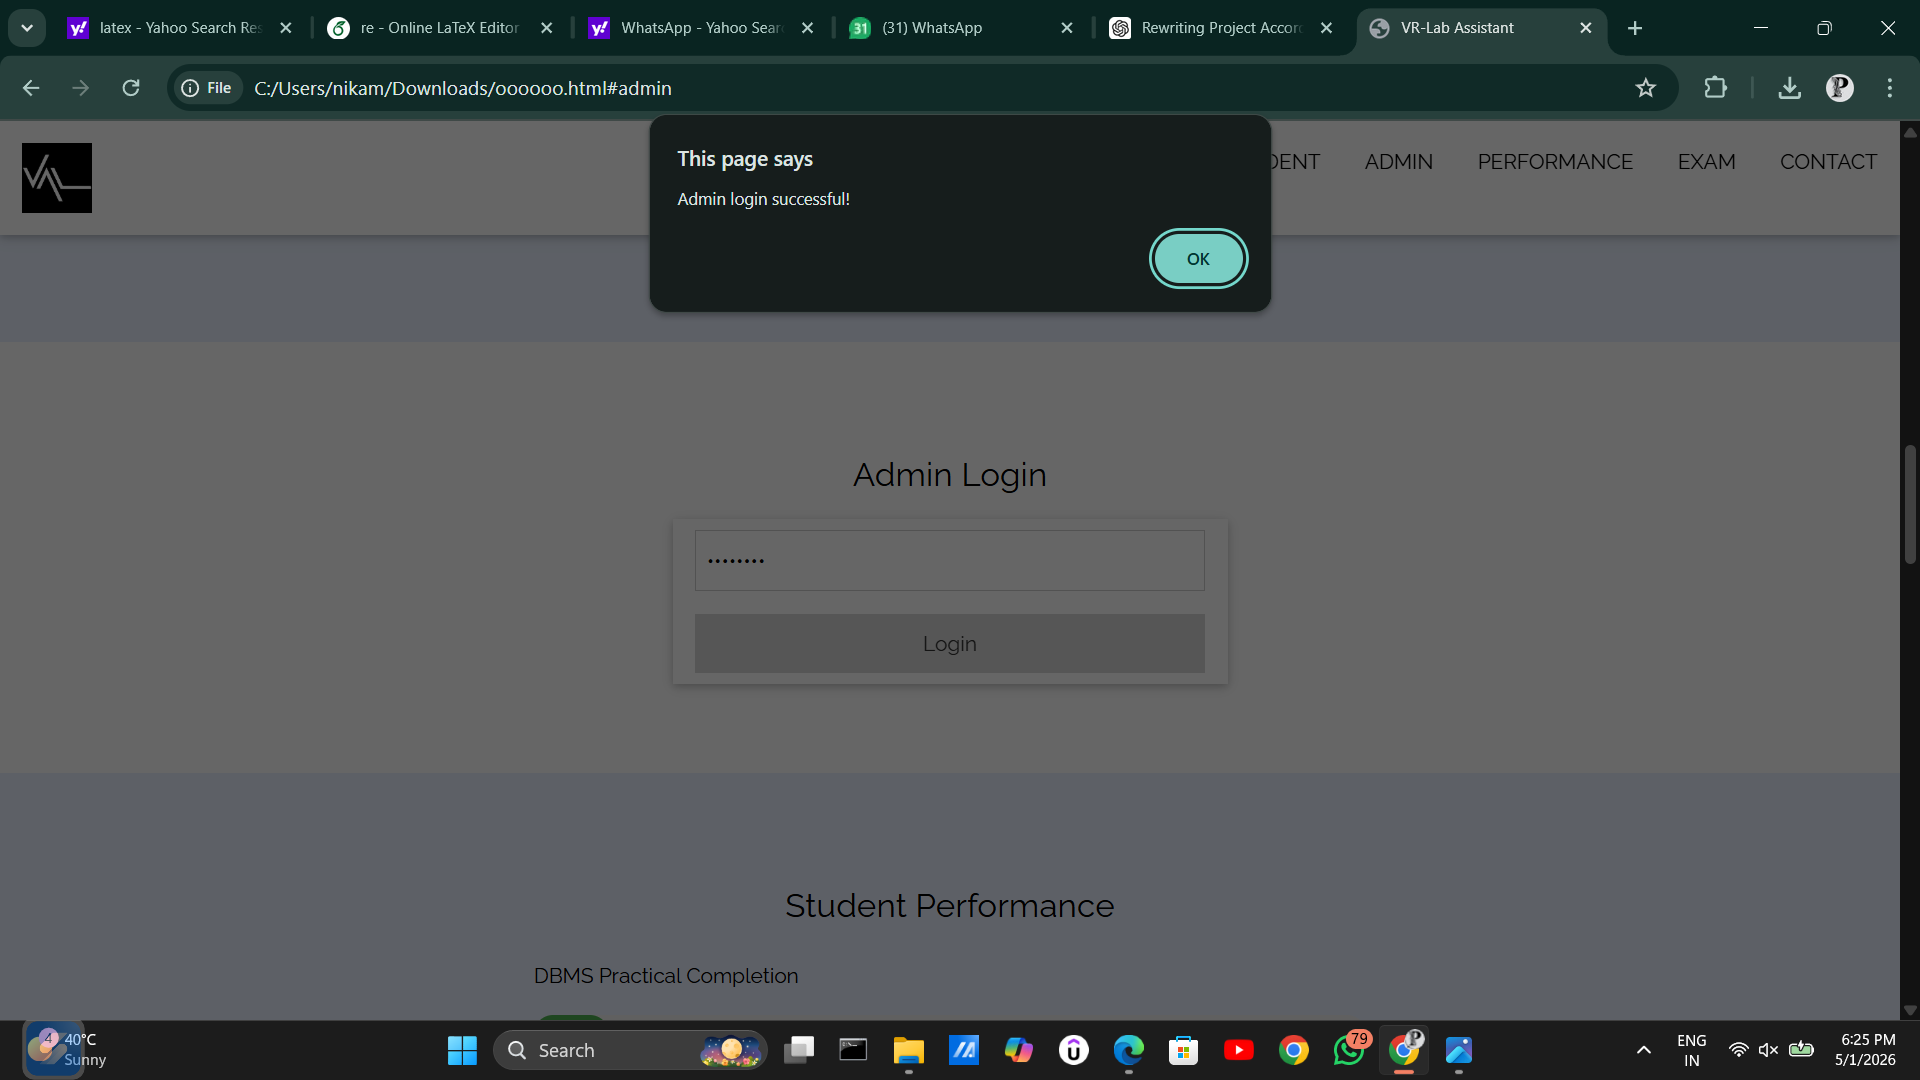
\includegraphics[width=16cm,height=300]{chapters/adminlogin.png}
    \caption{Admin Login}
\end{figure}

\begin{figure}[H]
    \centering
    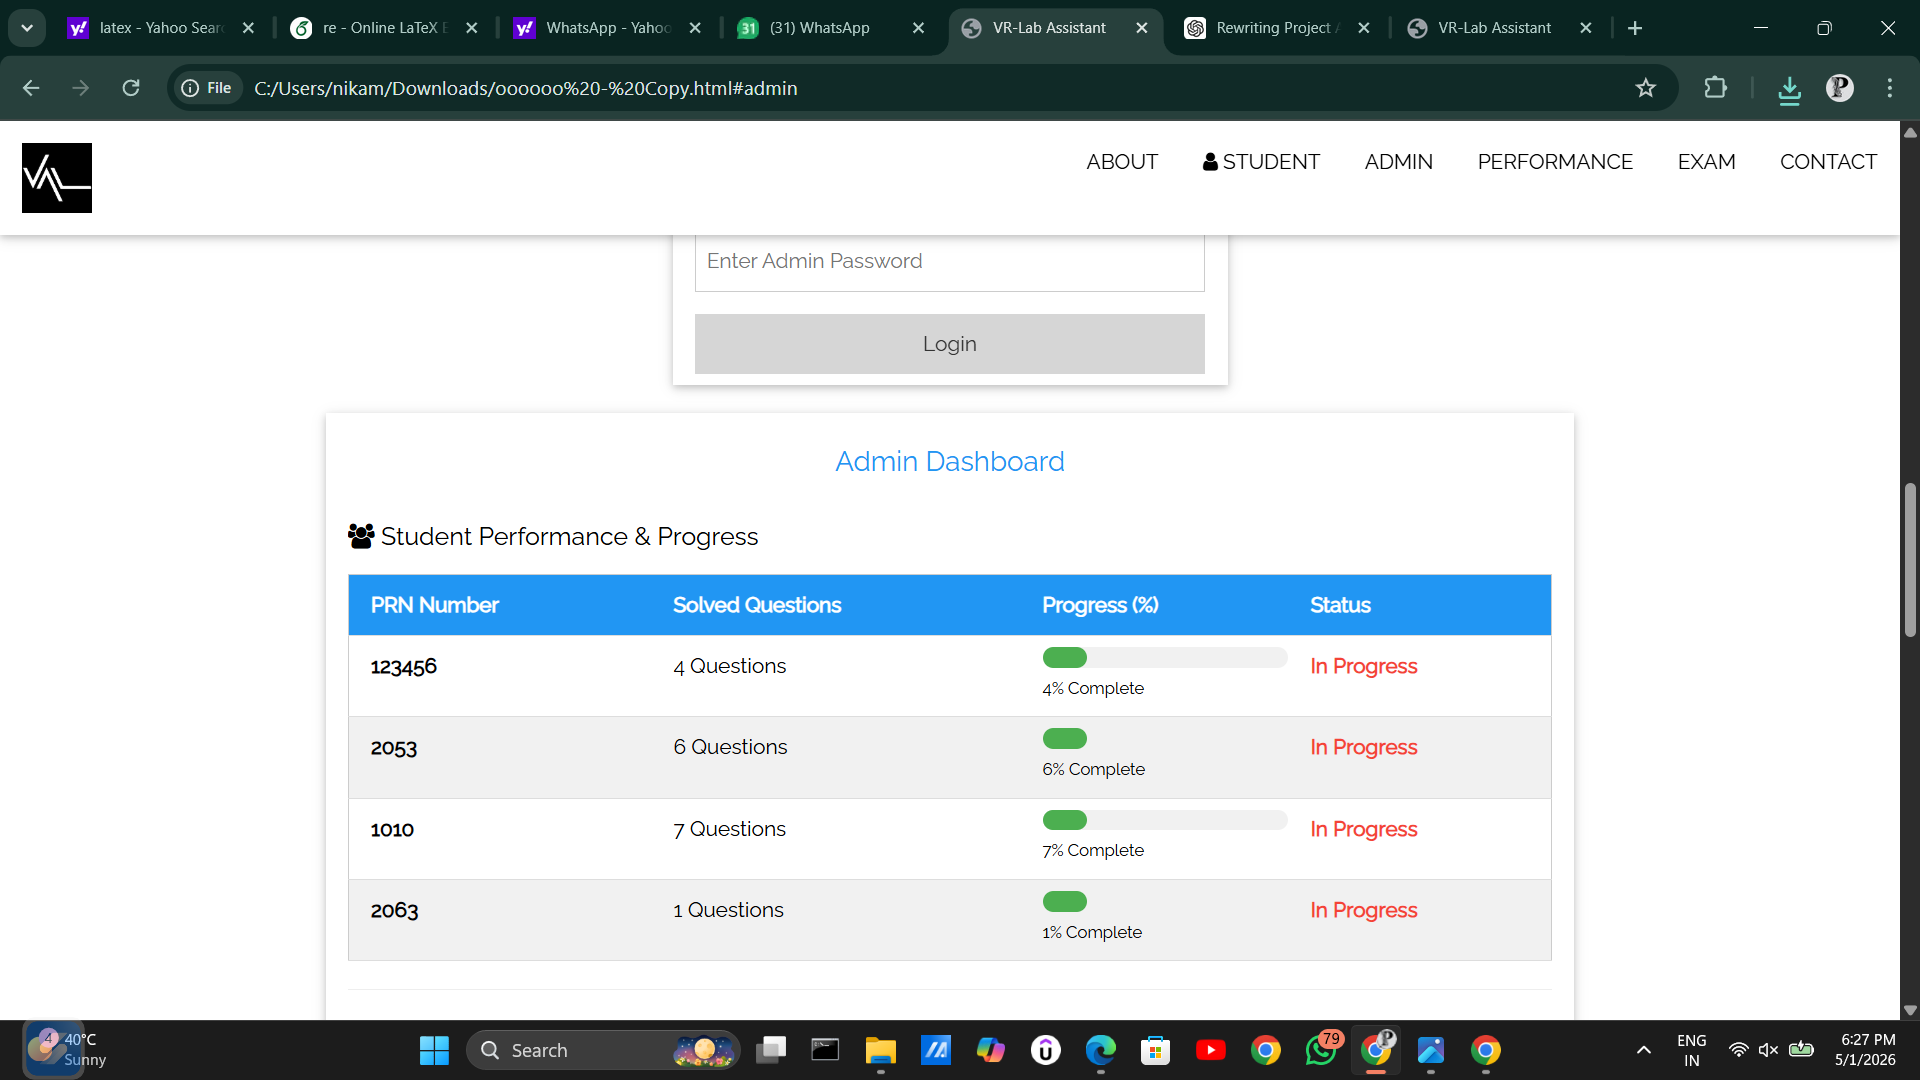
\includegraphics[width=16cm,height=300]{chapters/admindash.png}
    \caption{Admin Dashboared}
\end{figure}

\begin{figure}[H]
    \centering
    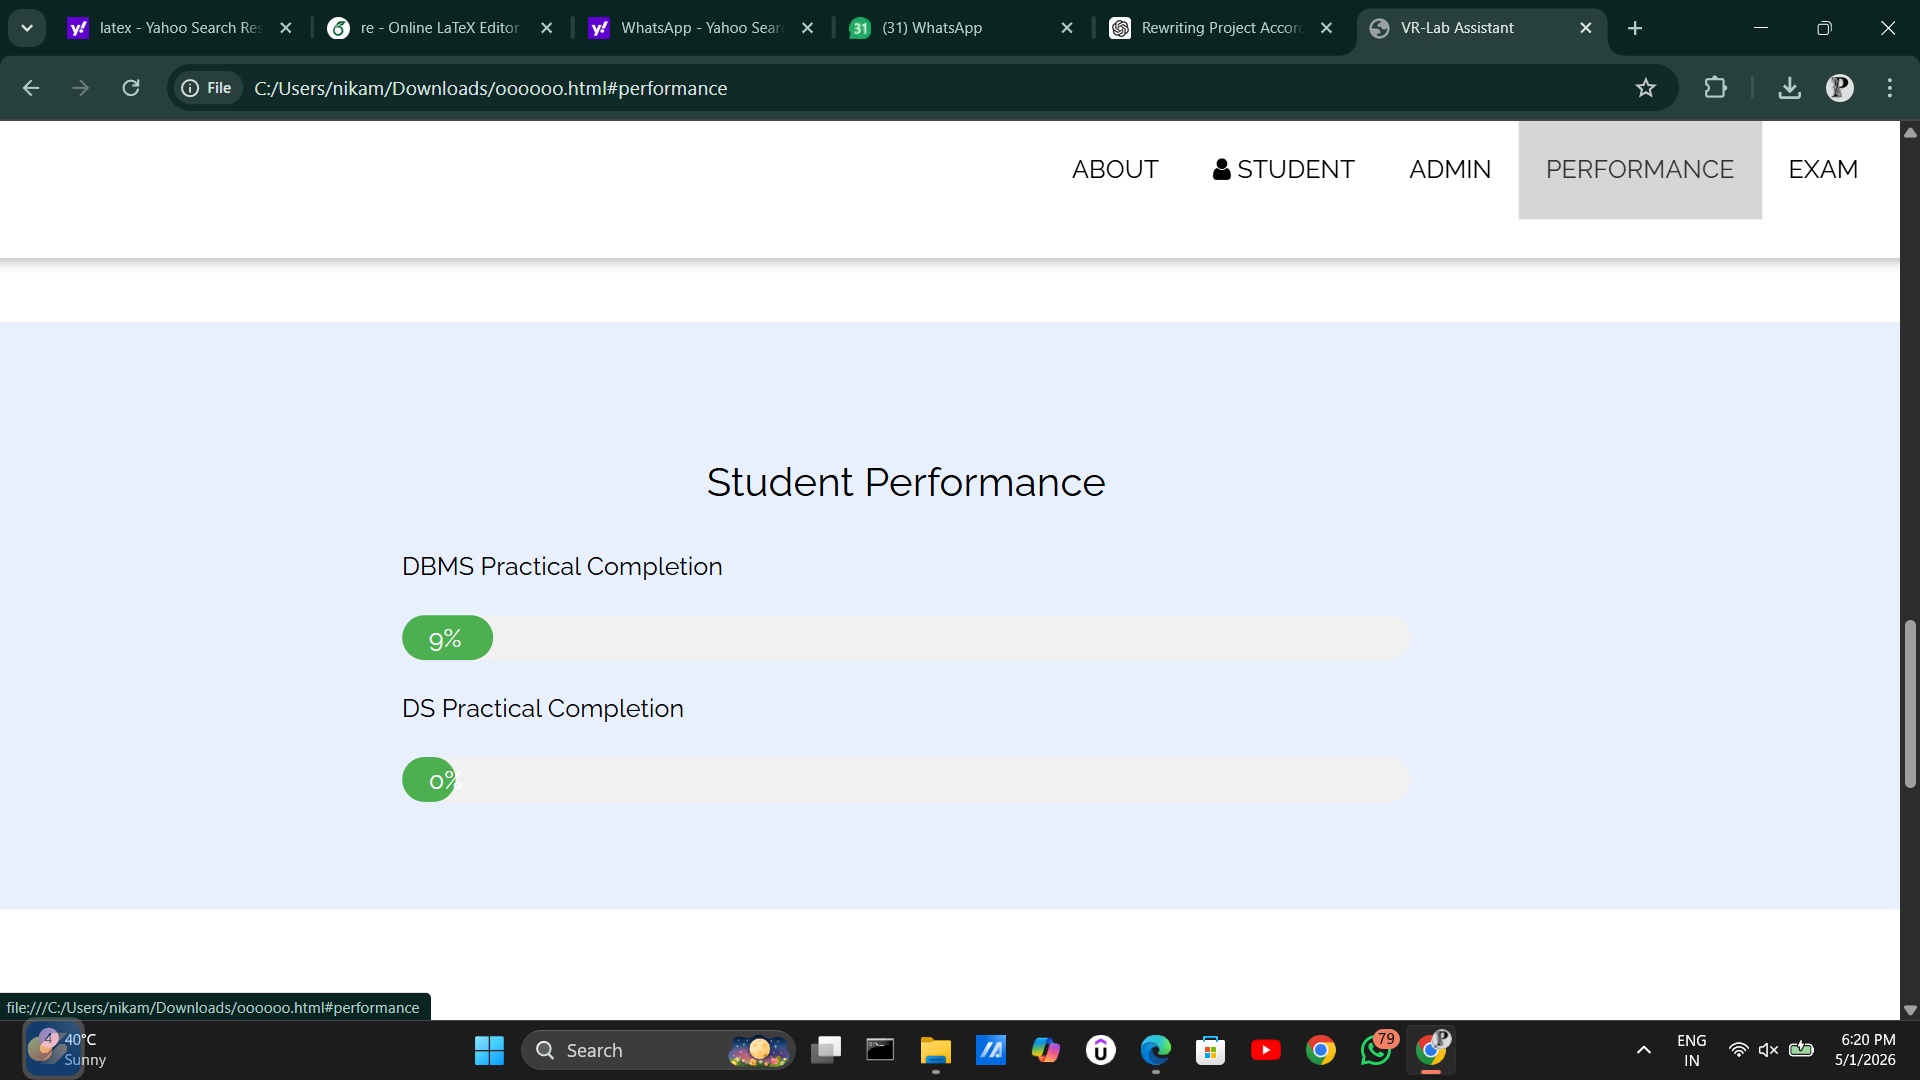
\includegraphics[width=16cm,height=300]{chapters/performance.png}
    \caption{Student Performance}
\end{figure}

\begin{figure}[H]
    \centering
    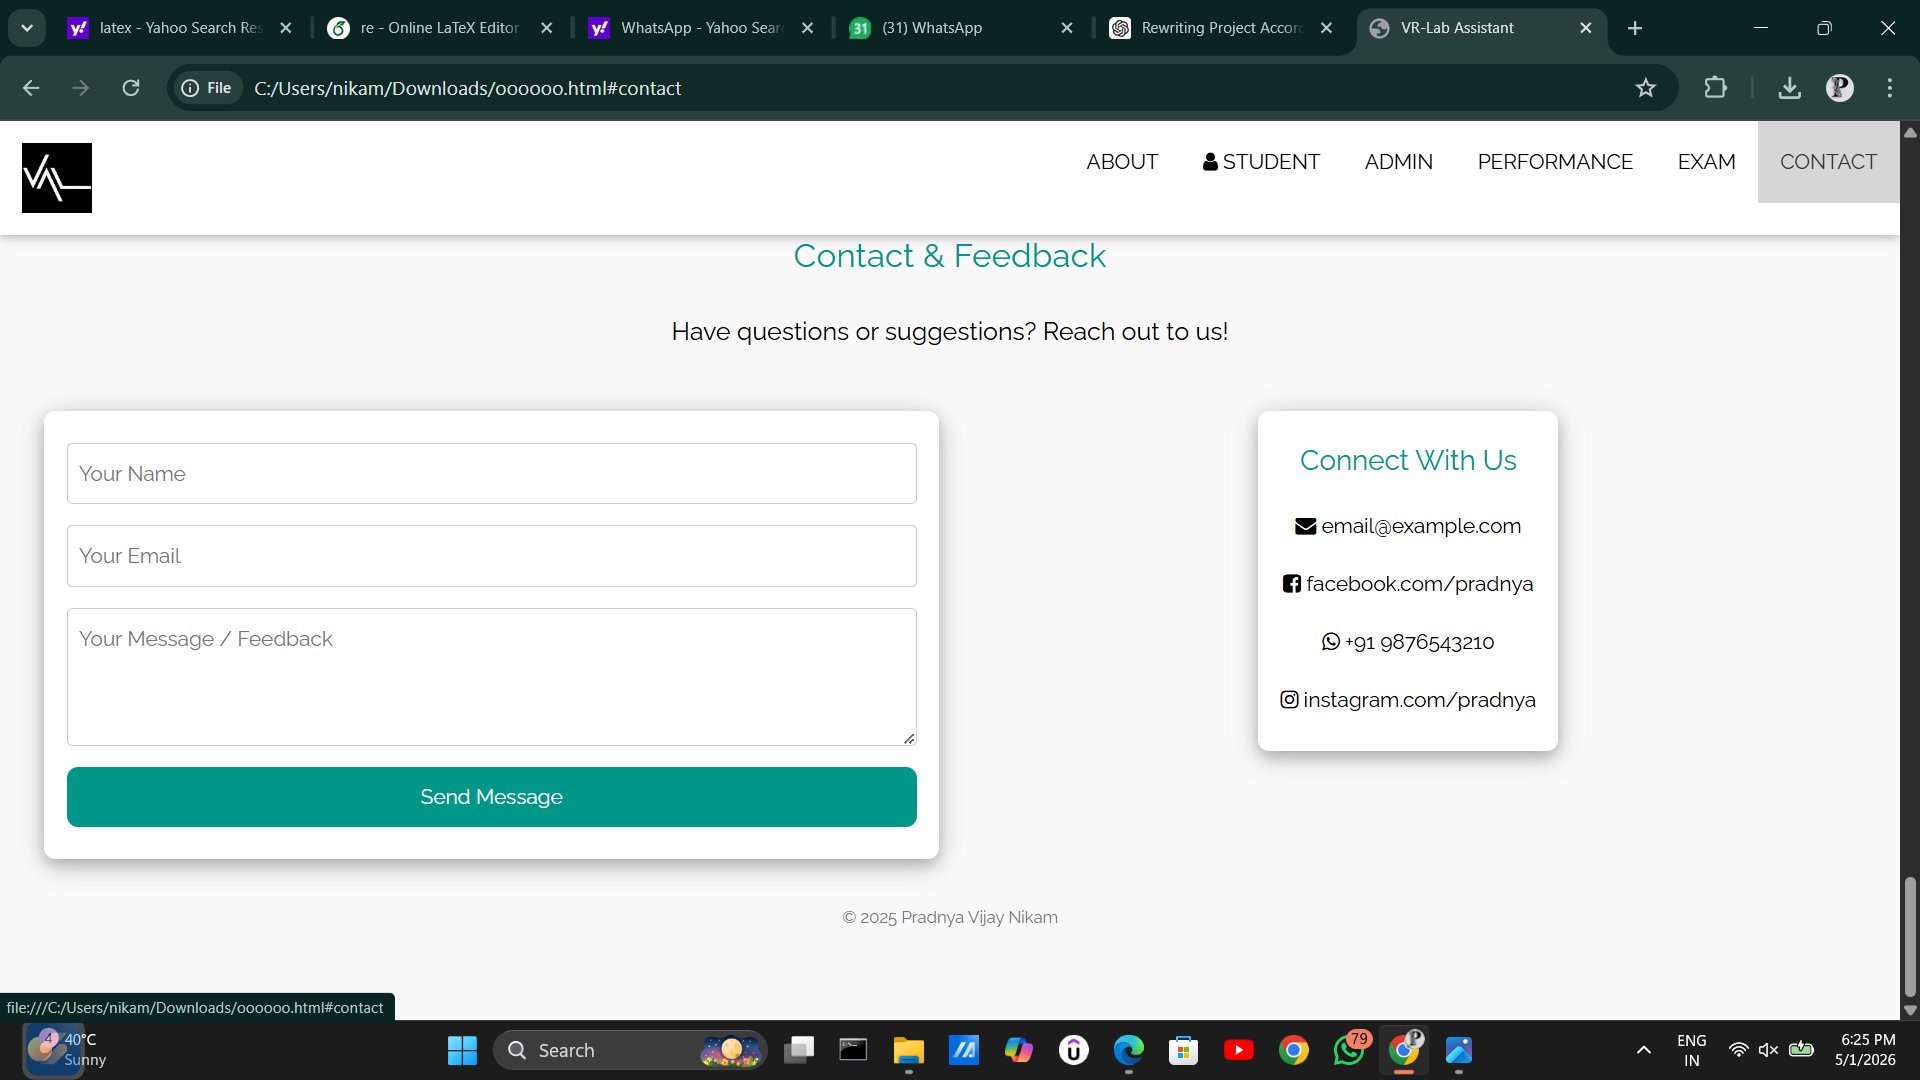
\includegraphics[width=16cm,height=300]{chapters/contact.png}
    \caption{Contact / Feedback Section}
\end{figure}

\begin{figure}[H]
    \centering
    
\includegraphics[width=16cm,height=300]{chapters/about.png}
    \caption{About Section}
\end{figure}
\end{document}
